\section{Background}
The initial research portion of this project focused on learning more about different remote situational awareness products and how they may have been improved using existing technology, eventually leading to a set of overall project goals.

\subsection{Remote Situational Awareness Products}
Many situational awareness devices consist of remote-controlled throwable robots with wireless video-streaming capability. One such example is the 110 FirstLook by Endeavor Robotics, seen in Figure \ref{robocop}a. This device is a throwable, rugged robot that streams real-time video of its surroundings, and is used to investigate dangerous locations and hazardous material while keeping its operator out of harm's way. The 110 FirstLook has four day and night cameras, and also supports two-way audio. The device is remotely controlled by a tablet operator control unit, and is currently in use for military applications \cite{endeavor}.
\par
Similar to the 110 FirstLook, the Bounce Image Explorer is a throwable camera ball that wirelessly transmits a 360$^\circ$ real-time video stream of its surroundings. The Bounce Image Explorer can be seen in Figure \ref{robocop}b. The Explorer processes input from six monochrome WVGA camera modules, and outputs a video stream that can be accessed from a tablet or smartphone. This device is currently in a trial phase with United States Law Enforcement \cite{bounceImaging}. 
\par
A more commercial remote situational awareness device is the Serveball Squito\textsuperscript{TM} \cite{serveball}. Squito is a wireless, throwable, 360$^{\circ}$ panoramic camera that implements target detection to produce a stabilized output video stream. This device is shown in Figure \ref{squito} below.

\begin{figure}[H]
	\centerline{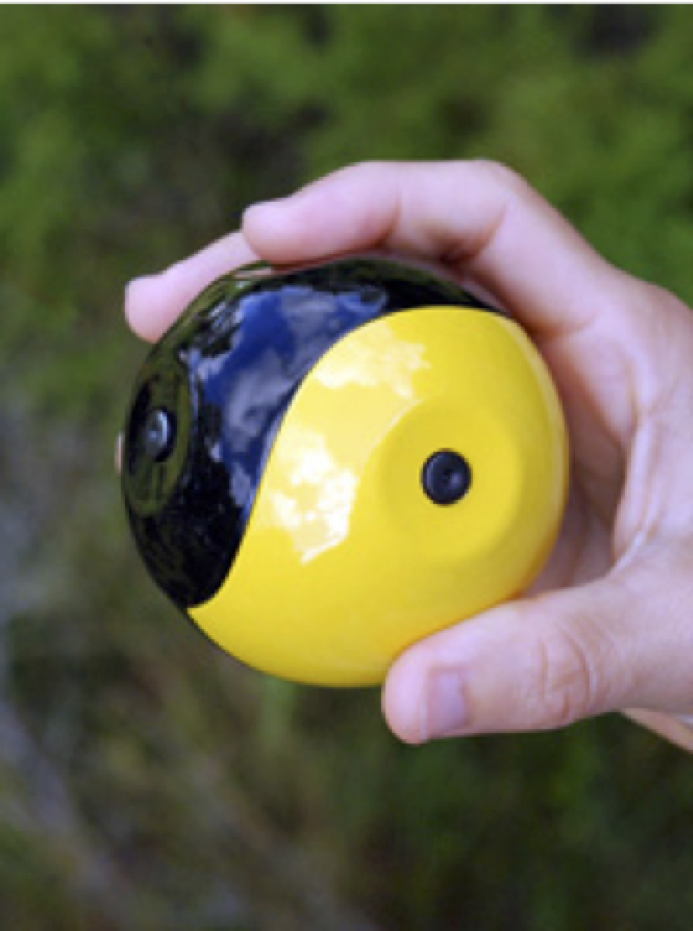
\includegraphics[width=0.3\textwidth]{serveball_squito.png}}
	\caption{Serveball's Squito \cite{serveball}}
	\label{squito}
\end{figure}

Squito utilizes a microprocessor receiving input from a fiber optic camera interface, as well as orientation and position sensors, in order to transmit a real-time stabilized video of its surroundings. The image in Figure \ref{squito_io} shows the input from the Squito's four camera inputs on the left, and a corresponding stitched output on the right. The device is still in the prototype stage, and has received interest from the first responder community. 
\par
\begin{figure}[H]
	\centerline{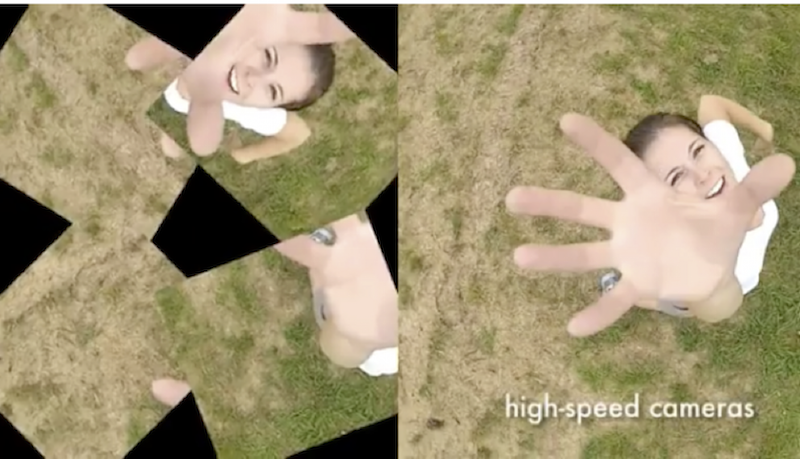
\includegraphics[width=0.6\textwidth]{serveball_io.png}}
	\caption{Serveball's Squito Input and Output \cite{serveball}}
	\label{squito_io}
\end{figure}
\par
The 110 FirstLook, Explorer, and Squito are all examples of remote situational awareness products that contain basic controls and real time video streaming outputs. Using additional image processing in the form of Simultaneous Localization and Mapping, the outputs of each of these devices could be improved to create comprehensive situational awareness. 

\subsection{Simultaneous Localization and Mapping}
As mentioned in the previous chapter, Simultaneous Localization and Mapping is the technique of mapping an unknown environment with respect to a localized agent. SLAM is especially useful for autonomous systems and remote observation, as it can be used for situational analysis and response. Recent research in the field of SLAM has focused on making these systems more portable.
\par
One application of such a system was a proof of concept of camera-based SLAM implementation for feature identification presented by Andrew Davison of Oxford University \cite{davison}. This system was handheld, and relied on a computer using a 2.2 GHz Pentium processor connected to a single camera and laser rangefinder. This system implemented edge detection on a known environment, and produced a real-time video output containing a 3D feature localization plot. An output frame from the device is shown in Figure \ref{rtSLAM}.

\begin{figure}[H]
	\centerline{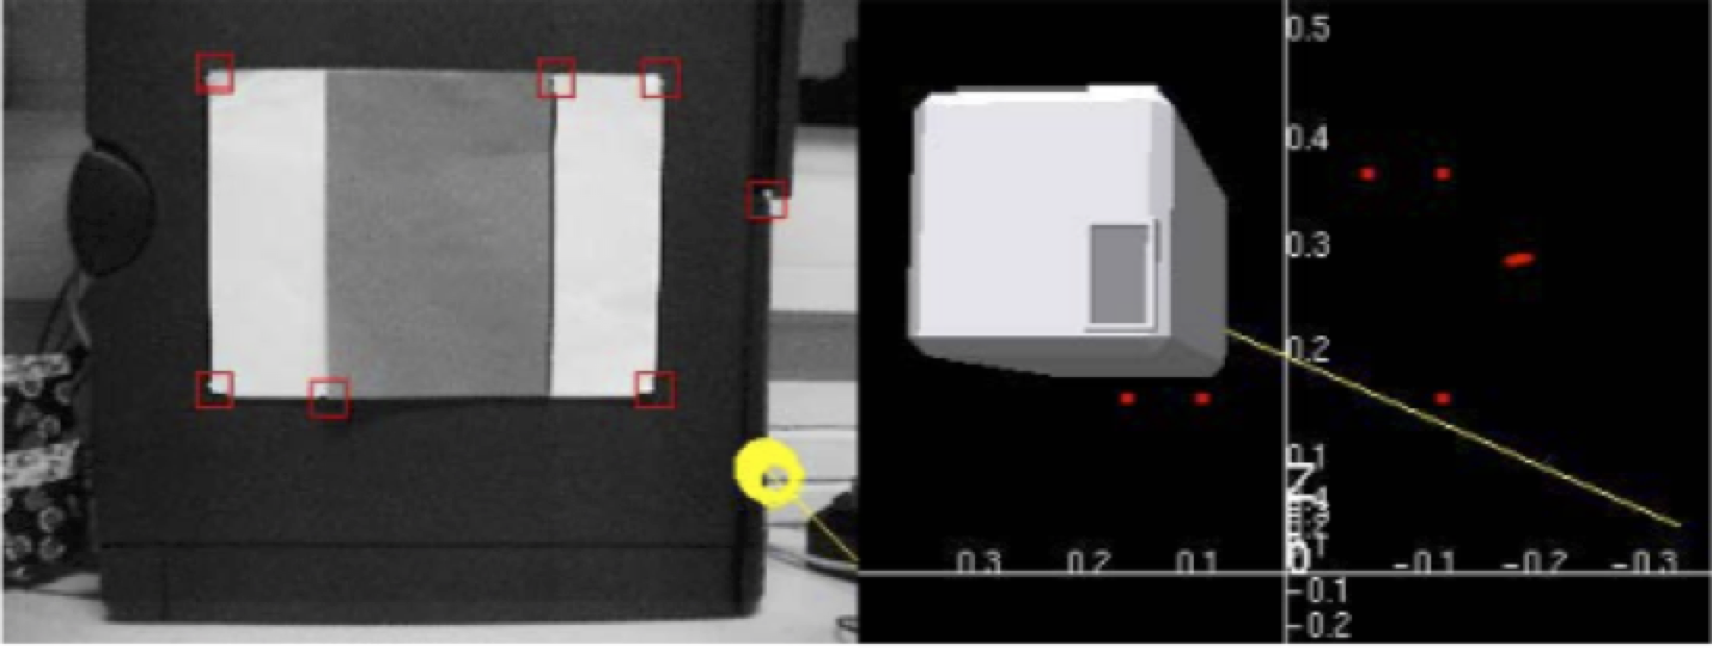
\includegraphics[width=0.8\textwidth]{real_time_SLAM.png}}
	\caption{Real-Time SLAM with a Single Camera \cite{davison}}
	\label{rtSLAM}
\end{figure}

The left image in Figure \ref{rtSLAM} shows 6 points of a paper target that were input to the system as prior knowledge, along with successfully marked identifying features (marked as red squares), and another identifying feature that was not marked for measurement (marked by a yellow circle). The frame on the right is a localization plot that displayed the relative positions of all red squares detected by the device.
\par
Along with identifying features of interest, SLAM image processing techniques are also used for depth estimation. The process of estimating depth from imagery is known as disparity mapping. Disparity mapping algorithms are used to calculate the similarities between stereo camera image pairs, and to convert said similarities to relative depth measurements. Disparity mapping is useful for situational awareness because it is used to determine the exact locations of all objects within a sensor suite's field of view.
\par
University of Bologna researchers Stefano Mattoccia and Matteo Poggi have worked to implement a real-time disparity mapping algorithm on an FPGA, and an example of a disparity image from this implementation is shown in Figure \ref{disparity_example} \cite{mattoccia}. Using their stereo disparity implementation, the researchers were able to generate real-time video showing the relative locations of objects within the device's field of view. The relative distance from the device to a given object was displayed using a color gradient, with nearer objects shown in brighter colors. Based on this depth information, it was also possible for the researchers to detect objects located within the field of view of the stereo imaging system, as shown in Figure \ref{disparity_example}. This implementation was extremely applicable to situational awareness systems, as it allowed for the localization of objects and creation of 2D slices of an area in real-time using only two camera sensors.
\par
\begin{figure}[H]
	\centerline{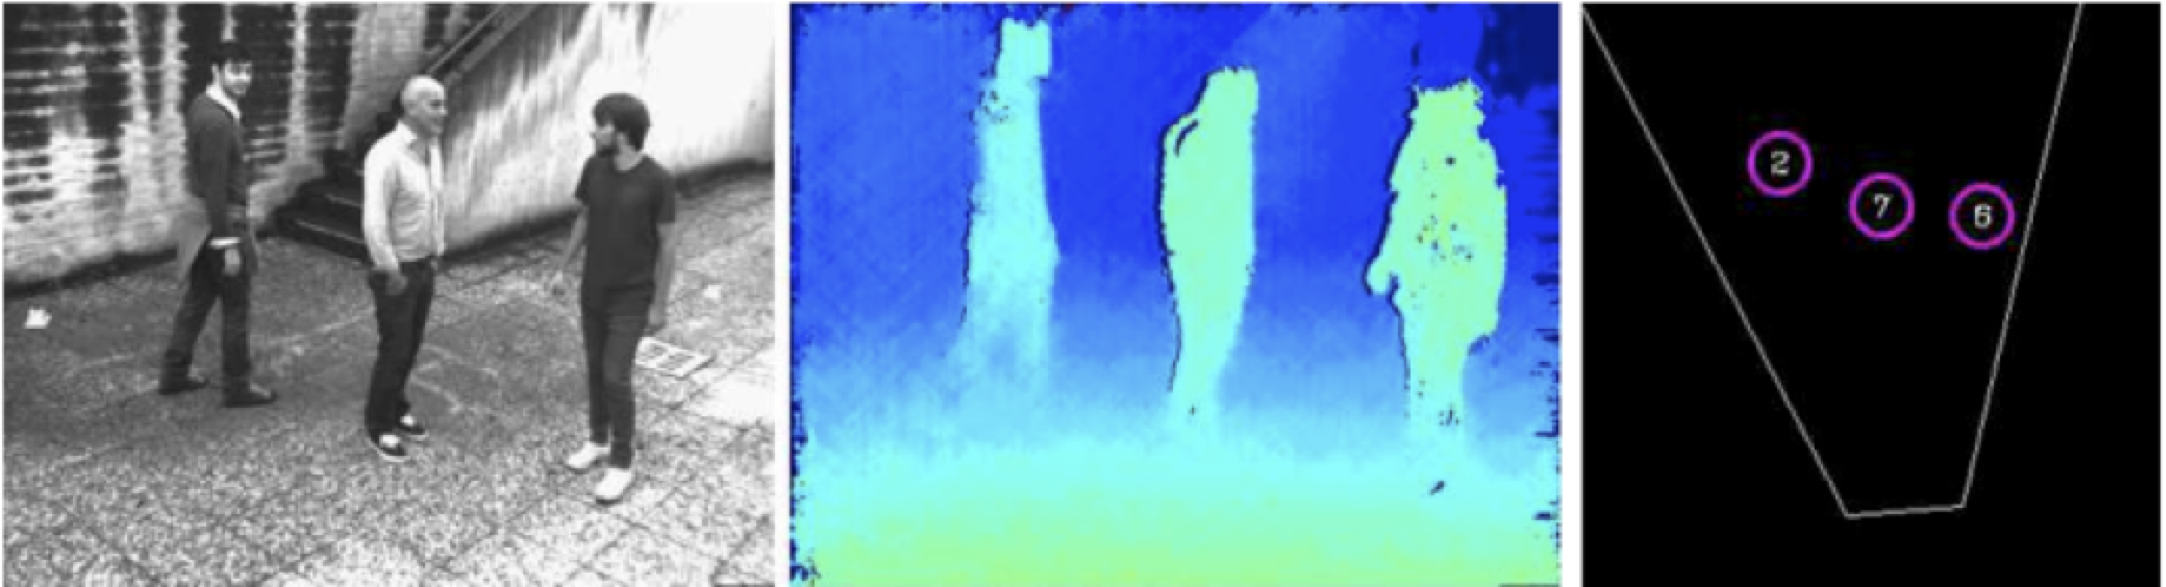
\includegraphics[width=0.9\textwidth]{disparity_example.png}}
	\caption{From Left to Right: Original Image, Disparity Map, Object Detection Results \cite{mattoccia}}
	\label{disparity_example}
\end{figure}
\par
A major concern with calculating disparity in real time is image processing speed. In the case of the implementation shown above, the parallelized data processing capabilities of FPGA hardware were used to address these concerns. The successful creation of this system demonstrated that FPGAs are useful for complex image processing applications \cite{mattoccia}. 

\subsection{The Zynq Evaluation and Development Board (ZedBoard)}
The FPGA platform used in this project was the Zynq Evaluation and Development Board, or ZedBoard. The ZedBoard is a low-cost development board containing a Xilinx Zynq-7000 All-Programmable SoC, and is shown in Figure \ref{zedboard_pic}.

\begin{figure}[H]
	\centerline{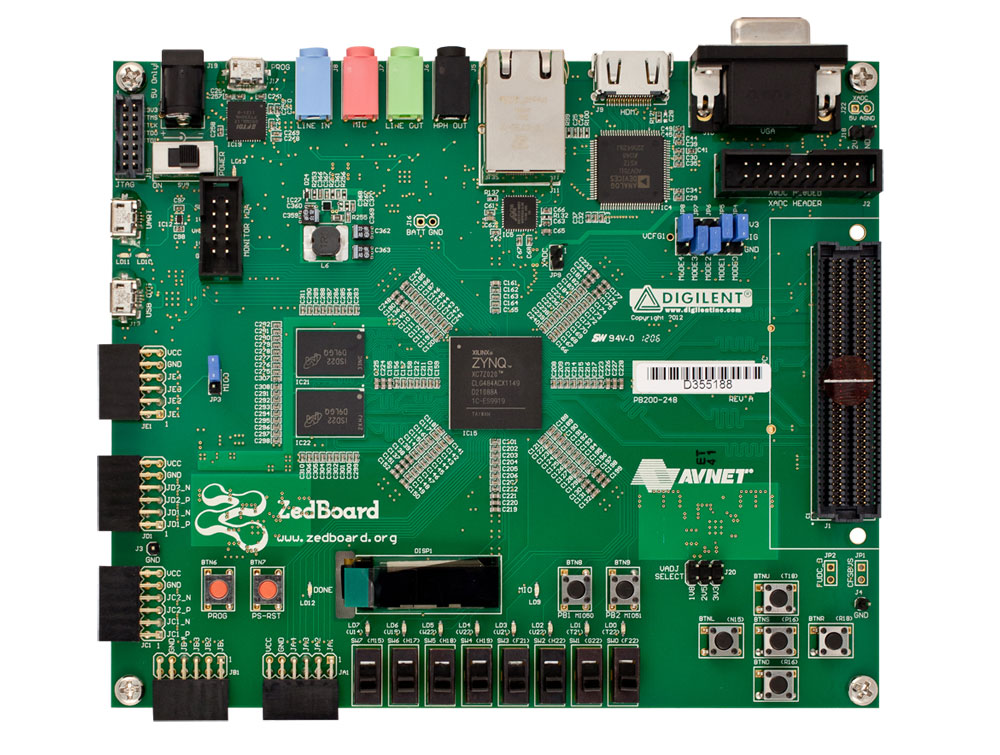
\includegraphics[width=1\textwidth]{ZedBoard.jpg}}
	\caption{The Avnet ZedBoard \cite{zedboard_photo}}
	\label{zedboard_pic}
\end{figure}

The Xilinx Zynq-7000 SoC consists of a dual-core ARM Cortex A9 processor coupled with Xilinx Artix-7 FPGA fabric. The ARM Cortex A9 processor uses a dedicated 33.3333 MHz clock source, while the onboard 100 MHz oscillator supplies the Programmable Logic (PL) clock. The Zynq-7000 SoC contains 85,000 programmable logic cells with 140 36K Block RAM modules. The ZedBoard also features 5 Pmod IO ports, 8 LEDs, 8 switches, 7 push buttons, a USB UART port, and a VGA port \cite{zedboard_datasheet}. These are shown in the ZedBoard's block diagram in Figure \ref{zedboardbd}.

\begin{figure}[H]
	\centerline{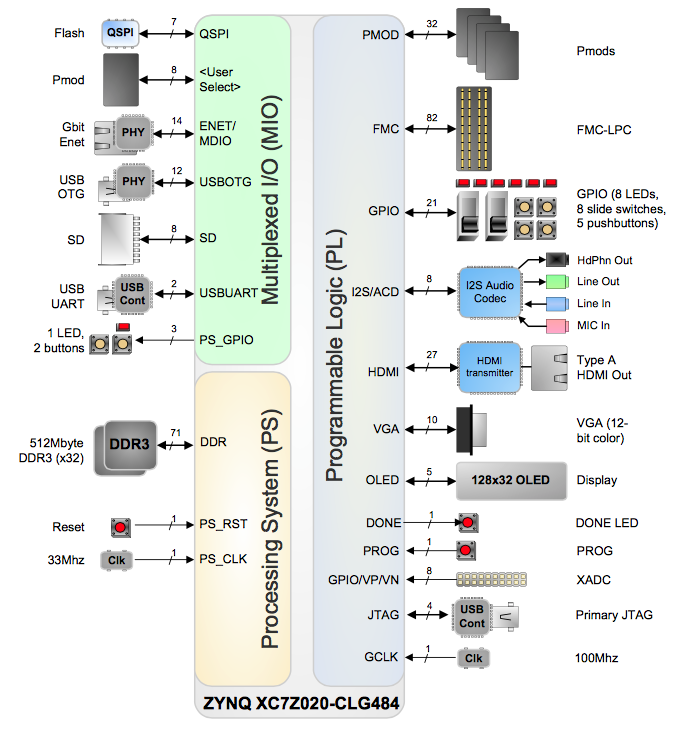
\includegraphics[width=0.85\textwidth]{ZedBoardBD.png}}
	\caption{ZedBoard Block Diagram \cite{zedboard_datasheet}}
	\label{zedboardbd}
\end{figure}
\par
As our research progressed, it became evident that FPGAs were a viable solution for implementing real-time situational awareness algorithms on a compact scale. For the purposes of this project, we decided to interface the ZedBoard with a stereo camera pair to gather disparity depth information on an area, and supplement that data with digital compass and rangefinder readings to produce detailed maps of the sensor suite's surroundings in real time. The implementation scheme for this device is detailed in the following chapter.





